\chapter{Suffix arrays}\label{ch:suffix-arrays}
Een tweede datastructuur die we in meer detail bekijken zijn suffix arrays.
We kiezen voor deze datastructuur verder te besturderen omdat ze geheugenefficiënter is dan een suffixboom, en bij deze datastructuur hebben we vastgesteld dat het geheugengebruik problematisch is.


\section{Wat zijn suffix arrays?}\label{sec:wat-zijn-suffix-arrays?}
Suffix arrays zijn een geheugenefficiëntere voorstelling van suffixbomen.
In plaats van een boomstructuur maken we hier gebruik van een array die de volgnummers van elke suffix in de originele string bevat.
Deze indexen worden lexicografisch gesorteerd.
Figuur~\ref{fig:suffixtree_vs_suffixarray} geeft een voorbeeld van een suffixboom en suffix array opgebouwd over de tekst \texttt{acacgt\$}.

\begin{center}
    \texttt{tekst: a|c|a|c|g|t|\$\\index: 0|1|2|3|4|5|6}
\end{center}
\begin{figure}[H]

    \begin{subfigure}[b]{0.6\linewidth}
        \resizebox{\linewidth}{!}{
            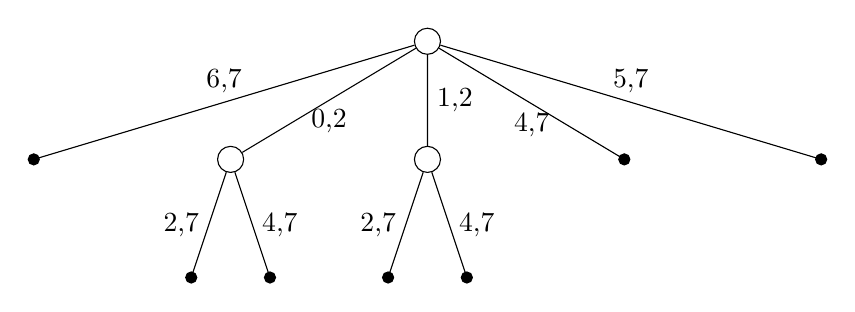
\begin{tikzpicture}
            [
                level 1/.style = {sibling distance = 2.5cm},
                level 2/.style = {sibling distance = 1cm}
            ]

                \node[draw, circle] {}
                child {
                    [fill] circle (2pt)
                    edge from parent node [above] {6,7}
                }
                child {
                    node[draw, circle] {}
                    child {
                        [fill] circle (2pt)
                        edge from parent node [left] {2,7}
                    }
                    child {
                        [fill] circle (2pt)
                        edge from parent node [right] {4,7}
                    }
                    edge from parent node [below] {0,2}
                }
                child {
                    node[draw, circle] {}
                    child {
                        [fill] circle (2pt)
                        edge from parent node [left] {2,7}
                    }
                    child {
                        [fill] circle (2pt)
                        edge from parent node [right] {4,7}
                    }
                    edge from parent node [right] {1,2}
                }
                child {
                    [fill] circle (2pt)
                    edge from parent node [below] {4,7}
                }
                child {
                    [fill] circle (2pt)
                    edge from parent node [above] {5,7}
                }
                ;
            \end{tikzpicture}
        }
        \caption{Suffixboom}
    \end{subfigure}
    \begin{subfigure}[b]{0.4\linewidth}
        \centering
        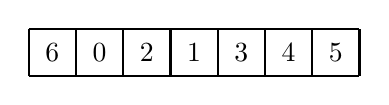
\begin{tikzpicture}[thick,scale=.6]
            \draw (0,0) grid (7,1);
            \path (.5,.5) node{$6$} foreach \i in {0,2,1,3,4,5} {++(1,0) node{$\i$}};
        \end{tikzpicture}
        \vspace{3em} % vertically center the array a bit
        \caption{Suffix array}
    \end{subfigure}

    \caption{Suffixboom en suffix array voor de string \texttt{acacgt\$}.}\label{fig:suffixtree_vs_suffixarray}
\end{figure}

Wanneer we de bladeren van de suffixboom van links naar rechts bekijken dan valt te zien dat dit overeen komt met de suffix array.
Dit is dan ook de link tussen deze twee datastructuren.
Onmiddellijk valt ook te zien dat een suffix array minder data bevat.
De interne knopen uit de suffixboom ontbreken namelijk, samen met de suffix links.
Indien deze informatie ook nodig is kan gebruik maakt worden van zogenaamde Enhanded Suffix Arrays (ESA).
Hierbij worden naast de suffix array nog 3 extra tabellen bijgehouden.
Deze worden de LCP, Child en suffix link table genoemd.


\section{Complixiteit}\label{sec:complixiteit}
Naïef kan het opbouwen van een suffix array in $O(n \log n)$ tijd en $O(n^2)$ geheugen gebeuren waarbij $n$ de lengte van de tekst is, dit aan de hand van traditionele sorteeralgoritmes zoals merge sort~\cite{mergeSort}.
Ondertussen bestaan er echter verschillende algoritmes die een tijdscomplexiteit van $O(n)$ bereiken~\cite{sais, ko_alura, radixSA, dark_archon, libdivsufsort}.
Bovendien vereisen deze veel minder geheugen dan een equivalente suffixboom.
Sommige implementaties vereisen slechts $5n + O(1)$ geheugen~\cite{dark_archon, libdivsufsort} met $n$ de lengte van de invoerstring.


\section{Bestaande implementaties}\label{sec:bestaande-implementaties}
Aangezien er meerdere erg geoptimaliseerde implementaties bestaan voor het opbouwen van een suffix array bekijken we eerst de performantie van deze implementaties.

% TODO: uitgevoerd op mac lokaal, vermeld dit nog ergens en voeg mac specs toe in de inleiding
\begin{table}[H]
    \centering
    \resizebox{\textwidth}{!}{
        \begin{tabular}{l l S[table-format=-2.2] S[table-format=-2.2] S[table-format=-1.2] S[table-format=-1.2]}
            Algoritme & Programmeertaal & \multicolumn{2}{c}{Tijd (in sec)} & \multicolumn{2}{c}{Geheugen (in GB)} \\
            \hline\hline
            &                      & {32 bit} & {64 bit} & {32 bit} & {64 bit} \\
            \cline{3-6}
            libdivsufsort  & C                    & 15.01    & 15.97    & 1.03     & 1.86     \\
            libdivsufsort  & Rust + bindings to C & 16.00    & 15.52    & 1.03     & 1.86     \\
            libdivsufsort  & Rust                 & 20.23    & {-}      & 1.03     & {-}      \\
            dark archon a4 & C                    & 39.34    & {-}      & 1.09     & {-}      \\
            libsais        & C                    & 6.38     & 6.46     & 1.03     & 1.86     \\
            radixSA        & C++                  & 9.74     & 11.26    & 2.11     & 3.52     \\
            \hline % TODO: de 2 gewone sais implementaties zijn hier nog niet vermeld, maar is ook niet direct een meerwaarde waarschijnlijk?
        \end{tabular}
    }
    \caption{}
    \label{tab:sa_building}
\end{table}

Aan de hand van bovenstaande tabel kunnen we concluderen dat de meest performante algoritmes op vlak van geheugengebruik libdivsufsort en libsais zijn.
Hierbij is er amper verschil in uitvoeringstijd tussen de 32 en 64 bit versies.
In het algemeen zijn de 64 bit versies een fractie trager.
Bovendien valt ook te zien dat het verschil tussen de C versie en Rust versie die bindings heeft naar de C code klein is.
De gemeten verschillen zijn namelijk eens in het voordeel van enkel de C code, en eens in het voordeel van de Rust code gebruik makende van C bindings.
Het verschil valt dus te verklaren door achtergrondprocessen.
Tot slot is libsais voor ons geval het algemeen beste algoritme.
Het geheugengebruik is minimaal en het is bovendien duidelijk het snelste algoritme.
Verder bevat het ook een implementatie dat gebruik maakt van 64 bit integers.
Dit is erg belangrijk voor onze usecase aangezien omdat de totale tekst die we willen indexeren (UniProtKB)langer is dan de maximale 32 bit integer.
Dit zorgt ervoor dat alle 32 bit integer implementaties onbruikbaar zijn voor ons einddoel.

\section{Toepassen van suffix arrays op een eiwitdatabank}\label{sec:toepassen-van-suffix-arrays-op-een-eiwitdatabank}
Het moeilijkste stuk van onze probleemstelling is het opbouwen van de suffix array.
Dit stuk kunnen we oplossen aan de hand van de algoritmes beschreven in sectie~\ref{sec:bestaande-implementaties}.
Eens we die suffix array opgebouwd hebben blijft er echter nog een stuk van ons probleem over.
Om te beginnen moeten we nog een mapping maken van de gevonden suffixen naar de bijbehorende proteïnes.
Op basis daarvan wordt daarna de LCA gezocht.

\subsection{Bouwen van de suffix array}
Zoals in de inleiding in sectie~\ref{sec:probleemstelling} willen we gebruik maken van Rust vanwege de combinatie van \textit{memory safety} en hoge performantie.
We willen echter gebruik maken van de hoge performantie die al verkregen is in sterk geoptimaliseerde, bestaande implementaties van algoritmes op een suffix array op te bouwen.
Daarom hebben we gekozen om gebruik te maken van de interoperabiliteit die bestaat tussen Rust en C/C++ code.
Om het ontwikkelen te beginnen hebben we er voor gekozen om gebruik te maken van bestaande Rust bindings\footnote{\url{https://crates.io/crates/libdivsufsort-rs}} naar de originele C implementatie van libdivsufsort~\cite{libdivsufsort}.
Ook al bleek uit het testen dat dit algoritme voor het opbouwen van de indexstructuur over een eiwitdatabank niet het snelste was, het geheugengebruik is wel minimaal.
\\ \\
Als tweede optie is er voor gekozen om zelf ook een simple Rust wrapper te schrijven rond de libsais C code.
Dit gebruik makende van het \texttt{bindgen}\footnote{\url{https://crates.io/crates/bindgen}} crate.
Op deze manier is het ook mogelijk om met weinig extra code gebruik te maken van deze snellere implementatie.
\\ \\
Het nadeel van het gebruiken van deze bindings naar C code is dat het oproepen van de effectieve C code gebeurd in een \texttt{unsafe} blok.
Hierbij is het dus mogelijk dat er geheugenfouten in het programma sluipen.
Dit risico is echter miniem aangezien dit vrij populaire, geteste bibliotheken zijn.
Bovendien zijn we ook zeker dat als een geheugenfout gebeurd dat dit aan de basis ervan zal liggen.
Dit is dus een afweging tussen optimale performantie (waar het wiel niet heruitgevonden wordt), en garantie van \textit{memory safety}.

\subsection{Mapping van suffix naar proteïne}\label{subsec:mapping-van-suffix-naar-proteine}
Deze mapping kan op 2 manieren gebeuren.
Een eerste optie is om expliciet voor elke suffix bij te houden bij welke proteïne die hoort.
Dit kan aan de hand van een array die even lang is als het aantal suffixen.
Het voordeel van deze aanpak is dat het vinden van de bijbehorende proteïne in $O(1)$ tijd kan.
\\ \\
De tweede optie is om enkel de eerste of laatste suffix per proteïne bij te houden.
Het voordeel van deze aanpak is dat er minder geheugen nodig is.
Er is hier $O(n)$ geheugen nodig met $n$ het aantal proteïnen, waar we bij de eerste aanpak $O(m)$ geheugen nodig hebben, met $m$ de lengte van de totale tekst.
Het nadeel is dan weer dat het vinden van de mapping trager is.
Bij deze implementatie duurt het $O(\log n)$ met $n$ het aantal proteïnes aan de hand van binair zoeken.

\subsection{Berekenen van de LCA}\label{subsec:berekenen-van-de-lca}
Zoals eerder vermeld bevat een suffix array geen informatie over de interne toppen die voorkomen bij een suffixboom.
Dit zorgt ervoor dat het niet mogelijk is om op basis hiervan de LCA van de organismen voor te berekenen voor al deze interne toppen.
In de plaats is dit nu iets dat \textit{on the fly} moet gebeuren tijdens het zoekproces zelf.
% TODO: we kunnen ook gebruik maken van enhanded suffix arrays en dat dan wel proberen doen, maar haalbaarheid daarvan is nog uit te zoeken.


\section{Sparse/Sampled suffix arrays}\label{sec:sparse/sampled-suffix-arrays}



